\documentclass[11pt]{beamer}\usepackage[]{graphicx}\usepackage[]{color}
%% maxwidth is the original width if it is less than linewidth
%% otherwise use linewidth (to make sure the graphics do not exceed the margin)
\makeatletter
\def\maxwidth{ %
  \ifdim\Gin@nat@width>\linewidth
    \linewidth
  \else
    \Gin@nat@width
  \fi
}
\makeatother

\definecolor{fgcolor}{rgb}{0.345, 0.345, 0.345}
\newcommand{\hlnum}[1]{\textcolor[rgb]{0.686,0.059,0.569}{#1}}%
\newcommand{\hlstr}[1]{\textcolor[rgb]{0.192,0.494,0.8}{#1}}%
\newcommand{\hlcom}[1]{\textcolor[rgb]{0.678,0.584,0.686}{\textit{#1}}}%
\newcommand{\hlopt}[1]{\textcolor[rgb]{0,0,0}{#1}}%
\newcommand{\hlstd}[1]{\textcolor[rgb]{0.345,0.345,0.345}{#1}}%
\newcommand{\hlkwa}[1]{\textcolor[rgb]{0.161,0.373,0.58}{\textbf{#1}}}%
\newcommand{\hlkwb}[1]{\textcolor[rgb]{0.69,0.353,0.396}{#1}}%
\newcommand{\hlkwc}[1]{\textcolor[rgb]{0.333,0.667,0.333}{#1}}%
\newcommand{\hlkwd}[1]{\textcolor[rgb]{0.737,0.353,0.396}{\textbf{#1}}}%

\usepackage{framed}
\makeatletter
\newenvironment{kframe}{%
 \def\at@end@of@kframe{}%
 \ifinner\ifhmode%
  \def\at@end@of@kframe{\end{minipage}}%
  \begin{minipage}{\columnwidth}%
 \fi\fi%
 \def\FrameCommand##1{\hskip\@totalleftmargin \hskip-\fboxsep
 \colorbox{shadecolor}{##1}\hskip-\fboxsep
     % There is no \\@totalrightmargin, so:
     \hskip-\linewidth \hskip-\@totalleftmargin \hskip\columnwidth}%
 \MakeFramed {\advance\hsize-\width
   \@totalleftmargin\z@ \linewidth\hsize
   \@setminipage}}%
 {\par\unskip\endMakeFramed%
 \at@end@of@kframe}
\makeatother

\definecolor{shadecolor}{rgb}{.97, .97, .97}
\definecolor{messagecolor}{rgb}{0, 0, 0}
\definecolor{warningcolor}{rgb}{1, 0, 1}
\definecolor{errorcolor}{rgb}{1, 0, 0}
\newenvironment{knitrout}{}{} % an empty environment to be redefined in TeX

\usepackage{alltt}

\makeatletter
\def\maxwidth{ %
  \ifdim\Gin@nat@width>\linewidth
    \linewidth
  \else
    \Gin@nat@width
  \fi
}
\makeatother

\definecolor{shadecolor}{rgb}{.97, .97, .97}
\definecolor{messagecolor}{rgb}{0, 0, 0}
\definecolor{warningcolor}{rgb}{1, 0, 1}
\definecolor{errorcolor}{rgb}{1, 0, 0}

\usepackage{alltt}
\usepackage{natbib}
\usepackage{array}
\usepackage[font=small,skip=5pt]{caption}
\usepackage{graphicx}
\usepackage{amsmath}
\usepackage{dsfont}
\usepackage[]{algorithm2e}
\usepackage{amsthm}
\usepackage{amsfonts}
\usepackage{url}
\usepackage{ulem}
\usepackage{afterpage}
\usepackage{bbm}
\usepackage{tikz}
\usepackage{amssymb}
\usepackage{bm}
\setbeamertemplate{caption}[numbered]

\usetheme{Warsaw}
\defbeamertemplate*{footline}{shadow theme}
{%
  \leavevmode%
  \hbox{\begin{beamercolorbox}[wd=.5\paperwidth,ht=2.5ex,dp=1.125ex,leftskip=.3cm plus1fil,rightskip=.3cm]{author in head/foot}%
    \usebeamerfont{author in head/foot}\insertframenumber\,/\,\inserttotalframenumber\hfill\insertshortauthor
  \end{beamercolorbox}%
  \begin{beamercolorbox}[wd=.5\paperwidth,ht=2.5ex,dp=1.125ex,leftskip=.3cm,rightskip=.3cm plus1fil]{title in head/foot}%
    \usebeamerfont{title in head/foot}\insertshorttitle%
  \end{beamercolorbox}}%
  \vskip0pt%
}

\setbeamertemplate{headline}{%
\leavevmode%
  \hbox{%
    \begin{beamercolorbox}[wd=\paperwidth,ht=2.5ex,dp=1.125ex]{palette quaternary}%
    \insertsectionnavigationhorizontal{\paperwidth}{\hskip0pt plus1filll}{\hskip0pt plus1filll}
    \end{beamercolorbox}%
  }
}

\newcounter{saveenumi}
\newcommand{\seti}{\setcounter{saveenumi}{\value{enumi}}}
\newcommand{\conti}{\setcounter{enumi}{\value{saveenumi}}}
\resetcounteronoverlays{saveenumi}


\title[Online Updating of Variational Bayes]{Online Updating of Variational Bayes for Heterogeneous Forecasts of Vehicle Trajectory}
\author[Nathaniel Tomasetti]{Nathaniel Tomasetti}
\date{ }
\IfFileExists{upquote.sty}{\usepackage{upquote}}{}
\IfFileExists{upquote.sty}{\usepackage{upquote}}{}

\AtBeginSection[]{
  \begin{frame}
  \vfill
  \centering
  \begin{beamercolorbox}[sep=8pt,center,shadow=true,rounded=true]{title}
    \usebeamerfont{title}\insertsectionhead\par%
  \end{beamercolorbox}
  \vfill
  \end{frame}
}

\begin{document}

\begin{frame}
\titlepage
\centering
Supervised by Catherine Forbes and Anastasios Panagiotelis
\end{frame}


\begin{frame}
\tableofcontents
\end{frame}

\section{Background}
\subsection{Motivation}

\begin{frame}
\frametitle{Motivation}
\begin{itemize}
\item We aim to build a framework to provide density forecasts for new units in a hierarchy as they are observed.
\pause
\item Bayesian Inference in Forecasting:
\begin{enumerate}
\item Provides density forecasts for the variable of interest.
\item Provides a mechanism to update posterior distributions
\item Is easy to extend to hierarchical models.
\end{enumerate}
\pause
\vspace{3mm}
\item Bayesian Inference is only as good as its compuation:
\begin{enumerate}
\item Computation based on Markov Chain Monte Carlo (MCMC) is 'exact', but slow.
\item Computation based on Variational Bayes (VB) is fast, but approximate.
\end{enumerate}
\end{itemize}
\end{frame}

\begin{frame}
\frametitle{Motivation}
\begin{itemize}
\item We focus on Hierarchical Models where:
\begin{enumerate}
\item Each unit is a time series,
\item Inference conditioned on existing units in the hierarchy is available,
\item Inference conditioned on additional units in a short time-frame is desired.
\end{enumerate}
\vspace{3mm}
\pause
\item We aim to infer, and forecast, additional units as they are observed.
\pause
\item We want to leverage the existing information to improve the forecasts.
\end{itemize}
\end{frame}

\subsection{Bayesian Hierarchical Models}

\begin{frame}
\frametitle{Bayesian Hierarchical Models}
\begin{itemize}
\item Hierarchical Models are structured into three levels:
\begin{enumerate}
\item The likelihood: $p(z_i | \theta_i)$ for each unit $i$ in the model,
\item The prior: $p(\theta_i | \beta)$ where $\beta$ is shared across all $i$,
\item The hyper-prior: $p(\beta)$ is fixed.
\end{enumerate}
\pause
\vspace{5mm}
\item For $i = 1, 2, \dots, N$, we assume that the posterior distribution $$p(\beta, \theta_1, \dots, \theta_N | z_1, \dots, z_N)$$ is available.
\end{itemize}
\end{frame}

\begin{frame}
\frametitle{Bayesian Hierarchical Models}
\begin{itemize}
\item What about $i = N+1$? Using $\textbf{z}_{1:j} = \{z_i | i = 1, \dots, j\}$, $$p(\theta_{N+1} |\textbf{z}_{1:N+1}) \propto p(z_{N+1} | \theta_{N+1})\int_{\beta}p(\theta_{N+1} | \beta)p(\beta | \textbf{z}_{1:N})d\beta.$$
\pause
\item If there is a time constraint, we might use VB with the approximation $$p(\theta_{N+1} |\textbf{z}_{1:N+1}) \approx q_{\lambda}(\theta_{N+1} | \textbf{z}_{1:N+1})$$
\item choosing $$\lambda_{VB} = \arg \underset{\lambda}{\min}\mbox{ }D(p, q).$$
\end{itemize}
\end{frame}

\subsection{Variational Bayes}

\begin{frame}[label=VB]
\frametitle{Variational Bayes}
\begin{itemize}
\item Typically minimize the Kullback-Leibler Divergence from $q$ to $p$,
\begin{align*}
\label{KL-def}
KL[q_{\lambda}(\theta_{N+1} &| \textbf{z}_{1:N+1})\hspace{.1cm}||\hspace{.1cm}p(\theta_{N+1} | \textbf{z}_{1:N+1})] = \\
&E_q \left[ \log(q_{\lambda}(\theta_{N+1} | \textbf{z}_{1:N+1})) - \log(p(\theta_{N+1} | \textbf{z}_{1:N+1})) \right],
\end{align*}
\item Maximising the Evidence Lower Bound (ELBO) is a tractable alternative, $$\mathcal{L}(q, \lambda) = E_{q} \left[\log(p(\theta_{N+1}, \textbf{z}_{1:N+1})) - \log(q_{\lambda}(\theta | \textbf{z}_{1:N+1}))\right],$$
\pause
\item For a fixed family $q$, find optimal $\lambda$ with \hyperlink{SGA}{gradient ascent}:
\begin{equation*}
\lambda^{(m+1)} = \lambda^{(m)} + \rho^{(m)} \widehat{\frac{\partial\mathcal{L}(q, \lambda)}{\partial \lambda}} \bigg\rvert_{\lambda = \lambda^{(m)}}
\end{equation*}
\end{itemize}
\end{frame}

\begin{frame}
\frametitle{Stochastic Optimisation}
\begin{itemize}
\item ELBO gradients can be estimated by the Score Estimator:
\begin{align*}
\widehat{\frac{\partial\mathcal{L}(q, \lambda)}{\partial \lambda}}_{SC} &= \sum_{j = 1}^M \frac{\partial \log(q_{\lambda}(\theta_{N+1}^{(j)} | \textbf{z}_{1:N+1}))}{\partial \lambda}  \\
&\times \left(\log(p(\theta_{N+1}^{(j)}, \textbf{z}_{1:N+1})) - \log(q_{\lambda}(\theta_{N+1}^{(j)} | \textbf{z}_{1:N+1})) \right),
\end{align*}
where $\theta_{N+1}^{(j)} \sim q_{\lambda}(\theta_{N+1} | \textbf{z}_{1:N+1})$.
\end{itemize}
\end{frame}

\begin{frame}
\frametitle{Stochastic Optimisation}
\begin{itemize}
\item Or the Reparameterised Estimator, where $\epsilon = f^{-1}(\theta_{N+1}, \lambda)$:
\begin{align*}
\widehat{\frac{\partial\mathcal{L}(q, \lambda)}{\partial \lambda}}_{RP} &= \sum_{j = 1}^M \frac{\partial J(\lambda, \epsilon^{(j)})}{\partial \lambda} + \frac{\partial \theta_{N+1}}{\partial \lambda} \\
&\times \frac{\partial \log(p(\theta_{N+1}, \textbf{z}_{1:N+1}))}{\partial \theta_{N+1}} \bigg\rvert_{\theta_{N+1} = f(\lambda, \epsilon^{(j)})},
\end{align*}
where $\epsilon^{(j)} \sim q(\epsilon)$ and $J(\lambda, \epsilon)$ is the Jacobian of $f$.
\end{itemize}
\end{frame}

\section{Online Heterogeneous Forecasting: Problem}
\subsection{Self-Driving Vehicles}

\begin{frame}
\frametitle{Self-Driving Vehicles}
\begin{itemize}
\item Many major manufacturers expect consumer self-driving vehicles to be available in the next 2-5 years
\pause
\item Autonomous driving has three major steps:
\begin{enumerate}
\item Detect surrounding traffic,
\item Forecast surrounding traffic,
\item Navigate through safely.
\end{enumerate}
\item We contribute to the second step.
\end{itemize}
\end{frame}

\begin{frame}
\frametitle{Self-Driving Vehicles}
\begin{itemize}
\item The existing literature has three major categories:
\begin{enumerate}
\item \textbf{Constant Behaviour Models:} \cite{Gindele2010, Houenou2013, Bautista2017, Waymo2017}
\item \textbf{Predict Driver State:} \cite{Forbes1995, Pentland1999, Kuge2000, Gindele2010, Geng2017}
\item \textbf{Provide Point Estimates:} \cite{Wolf2008, Ding2013, Woo2016b, Geng2017, Woo2017}
\end{enumerate}
\pause
\item Our approach:
\begin{enumerate}
\item Provides density forecasts of vehicle trajectory,
\item Incorporates driver heterogeneity,
\item Provides feasible inference for online vehicle data.
\end{enumerate}
\end{itemize}
\end{frame}

\begin{frame}
\frametitle{Forecasting Approach}
\begin{itemize}
\item \textbf{Training Vehicle} data is collected during development of the self-driving vehicle.
\item \textbf{Test Vehicles} are encountered while driving and require forecasts.
\begin{figure}
\centering
\includegraphics[width = \textwidth]{problem}
\end{figure}
\end{itemize}
\end{frame}

\subsection{The Next Generation Simulation Dataset}

\begin{frame}
\frametitle{Next Generation Simulation Data}
\begin{itemize}
\item The US Federal Highway Administration filmed 6101 vehicles every 100 milliseconds on the US 101 Freeway.
\item We model and remove the curvature from the dataset.
\begin{figure}
\centering
\includegraphics[width = \textwidth]{roadStraightening}
\end{figure}
\end{itemize}
\end{frame}

\begin{frame}
\frametitle{Trigonometric Motion Equations}
\begin{itemize}
\item Changes in position are the result of velocity $v$ and steering angle $\delta$,
\begin{align}
x^*_{i, t} &= x^*_{i, t-1} + v_{i, t} \cos(\delta_{i, t}) \label{xEq}, \\
y^*_{i, t} &= y^*_{i, t-1} + v_{i, t} \sin(\delta_{i, t}) \label{yEq}.
\end{align}
\begin{figure}
\centering
\includegraphics[width = 0.7\textwidth]{motion}
\end{figure}
\end{itemize}
\end{frame}

\begin{frame}
\frametitle{Extracting Driver Inputs}
\begin{itemize}
\item Transform the data to driver actions:
\end{itemize}
\begin{align}
\delta_{i, t} &= 
     \begin{cases}
       \tan^{-1}\left(\frac{(y^*_{i, t} - y^*_{i, t-1})}{(x^*_{i, t} - x^*_{i, t-1})} \right)  &\quad\text{if }x^*_{i, t} \neq x^*_{i, t-1} \\
       \frac{\pi}{2} &\quad\text{if } y^*_{i, t} > y^*_{i, t-1} \mbox{ and } x^*_{i, t} = x^*_{i, t-1} \\
       -\frac{\pi}{2} &\quad\text{if } y^*_{i, t} < y^*_{i, t-1} \mbox{ and } x^*_{i, t} = x^*_{i, t-1} \\
       \delta_{i, t-1} &\quad\text{otherwise,} \\ 
     \end{cases} \label{dEq} \\
v_{i, t} &= \sqrt{(x^*_{i, t} - x^*_{i, t-1})^2 + (y^*_{i, t} - y^*_{i, t-1})^2} \label{vEq}, \\
a_{i, t} &= v_{i, t} - v_{i, t-1}. \label{aEq}
\end{align}
\end{frame}

\begin{frame}
\frametitle{Vehicle Acceleration and Angle}
\begin{figure}
\includegraphics[width = \textwidth]{timeSeries}
\end{figure}
\end{frame}

\subsection{Auto-Regressive Models for Trajectory Forecasting}

\begin{frame}
\frametitle{Auto-Regressive Models for Trajectory Forecasting}
\begin{figure}
\centering
\includegraphics[width = \textwidth]{pacf2}
\end{figure}
\begin{itemize}
\item Dynamics are modelled with bivariate AR processes.
\pause
\item We consdier three approaches:
\begin{enumerate}
\item The Homogeneous Model
\item The Independent Heterogeneous Model
\item The Clustered Heterogeneous Model
\end{enumerate}
\end{itemize}
\end{frame}

\begin{frame}
\frametitle{The Homogeneous Approach}
\begin{itemize}
\item Acceleration and Angle are modelled independently:
\begin{align}
a_{i, t} &= \sum_{j = 1}^p \phi_{j} a_{i, t-j} + \sigma_{\epsilon} \epsilon_{i, t}, \label{aAR} \\
\delta_{i, t} &= \pi/2 + \sum_{j = 1}^q \gamma_{j} (\delta_{i, t-j} - \pi/2) + \sigma_{\eta} \eta_{i, t}. \label{dAR} 
\end{align}
\pause
\item Collect parameters:
\begin{align}
\theta &= \{\phi_{1}, \dots, \phi_{p}, \gamma_{1}, \dots, \gamma_{q}, \log(\sigma^{2}_{\epsilon}), \log(\sigma^{2}_{\eta})\}. \label{thetaVec} \\
\theta &\sim \mathcal{N}\left(\mu, \Sigma \right) \label{indPrior} 
\end{align}
\item Parameters are shared across different vehicles.
\end{itemize}
\end{frame}

\begin{frame}
\frametitle{The Independent Heterogeneity Model}
\begin{itemize}
\item Allow each vehicle to have an independent 
\item Each vehicle $i$ has an associated $\theta_i$:
\item Each $\theta_i$ has an identical, independent prior:
\begin{equation}
\theta_i \overset{iid}{\sim} \mathcal{N}\left(\mu, \Sigma \right). 
\end{equation}
\item Vehicle posteriors are independent.
\item The training set does not provide information about the test set.
\end{itemize}
\end{frame}

\begin{frame}
\frametitle{The Clustered Heterogeneity Model}
\begin{itemize}
\item Replace the independent prior with a hierarchical prior:
\begin{equation}
\theta_i | \beta  \overset{iid}{\sim} \sum_{j=1}^K \pi_j \mathcal{N}(\mu_j, \Sigma_j)
\end{equation}
\pause
\item The hyper-prior is:
\begin{align*}
\mu_j &\sim \mathcal{N}\left(\bar{\mu}_j, \Omega_j\right), \\
\Sigma_j &\sim \mbox{Inverse Wishart}\left(\tau_j, \Psi_j\right), \\
\boldsymbol{\pi} &\sim \mbox{Dirichlet}\left(\alpha_1 = \alpha_2 = \dots = \alpha_K\right).
\end{align*}
\end{itemize}
\end{frame}

\begin{frame}
\frametitle{The Clustered Heterogeneity Model}
\begin{itemize}
\item Test set vehicles depend on the train set vehicles through $\beta$.
\begin{equation}
\label{hierNewCar}
p(\theta_{N+1} | \textbf{z}_{1:N+1}) \propto p(z_{N+1} | \theta_{N+1}) \int_{\beta} p(\theta_{N+1} | \beta) p (\beta | \textbf{z}_{1:N}) d\beta.
\end{equation}
\pause
\item The $\beta$ posterior is precise for large $N$,
\begin{equation}
\label{hierNewCar2}
p(\theta_{N+1} | \textbf{z}_{1:N+1}) \propto p(z_{N+1} | \theta_{N+1}) p(\theta_{N+1} | \hat{\beta}).
\end{equation}
\end{itemize}
\end{frame}

\begin{frame}
\frametitle{Evidence of Heterogeneity in the Model Posteriors}
\begin{figure}
\centering
\includegraphics[width = \textwidth]{hierSingleKDE2}
\end{figure}
\begin{itemize}
\item Top: Kernel Density Estimate of $E(\theta_i | z_i)$ from the IH Model.
\item Bottom: $p(\theta_{N+1} | \textbf{z}_{1:N})$ from the CH Model.
\end{itemize}
\end{frame}

\section{Updating Variational Bayes}

\begin{frame}
\frametitle{Updating Variational Bayes}
\begin{itemize}
\item Inference for self-driving vehicles needs to be fast.
\item Inference cannot slow down as the amount of data increases.
\begin{figure}[ht]
\centering
\includegraphics[width = \textwidth]{timeUpdate}
\end{figure}
\item Need to update $q_{\lambda_S}(\theta_{N+1} | z_{N+1, 1:S})$ to $q_{\lambda_T}(\theta_{N+1} | z_{N+1, 1:T})$.
\end{itemize}
\end{frame}

\begin{frame}
\frametitle{Approximate Bayesian Updating}
\begin{itemize}
\item The Bayesian Update Equation: 
\begin{equation}
\label{updatePost}
p(\theta_{N+1} | z_{N+1, 1:T}) \propto p(z_{N+1, S+1:T} | \theta_{N+1})p(\theta_{N+1} | z_{N+1, 1:S}).
\end{equation}
\pause
\item Computation typically requires evaluating the joint distribution,
\begin{equation}
\label{updateJoint}
p(\theta_{N+1}, z_{N+1, 1:T}) = p(z_{N+1, S+1:T} | \theta_{N+1})p(\theta_{N+1} | z_{N+1, 1:S}).
\end{equation}
\pause
\item We use the VB approximation of the time $S$ posterior,
\begin{equation}
\label{ApproxJoint}
\hat{p}(\theta_{N+1},  z_{N+1, 1:T}) = p(z_{N+1, S+1:T} | \theta_{i})q_{\lambda_S}(\theta_{N+1} | z_{N+1, 1:S}).
\end{equation}
\item Source of additional error: How close $q$ is to $p$.
\end{itemize}
\end{frame}

\begin{frame}
\frametitle{Updating Gradient Estimators}
\begin{itemize}
\item The updating score estimator:
\begin{align*}
&\widehat{\frac{\partial\mathcal{L}(q, \lambda_T)}{\partial \lambda_T}}_{USC} = \sum_{j = 1}^M \frac{\partial \log(q_{\lambda_T}(\theta_{N+1}^{(j)} | z_{N+1, 1:T}))}{\partial \lambda_T}  \\
&\times \left(\log(\hat{p}(\theta_{N+1},  z_{N+1, 1:T})) - \log(q_{\lambda_T}(\theta_{N+1}^{(j)} | z_{N+1, 1:T})) \right)
\end{align*}
where $\theta_{N+1}^{(j)} \sim q_{\lambda_T}(\theta_{N+1} | z_{N+1, 1:T})$. 
\end{itemize}
\end{frame}

\begin{frame}
\frametitle{Updating Gradient Estimators}
\begin{itemize}
\item The updating reparameterised estimator:
\begin{align*}
&\widehat{\frac{\partial\mathcal{L}(q, \lambda_T)}{\partial \lambda_T}}_{URP} = \sum_{j = 1}^M \frac{\partial J(\lambda_T, \epsilon^{(j)})}{\partial \lambda_T} + \frac{\partial f(\lambda_T, \epsilon^{(j)})}{\partial \lambda_T} \\
&\times \frac{\partial \log(\hat{p}(\theta_{N+1},  z_{N+1, 1:T})}{\partial \theta_{N+1}} \bigg\rvert_{\theta_{N+1} = f(\lambda_T, \epsilon^{(j)})} 
\end{align*}
where $\epsilon^{(j)} \sim q(\epsilon)$.
\end{itemize}
\end{frame}

\section{OHF: Results}

\begin{frame}
\frametitle{Forecast Procedure}
\begin{itemize}
\item Inference on the training vehicles $i = 1, \dots 2000$ is available.
\item For each test vehicle $i = 2001, \dots, 3387$, 
\item For $T = 100, 110, \dots, 450$ and $h = 1, 2, \dots 30$:
\begin{enumerate}
\item Observe $z_{i, 1:T}$,
\item Infer $p(\theta_{i} | \textbf{z}_{1:N}, z_{i, 1:T})$,
\item Forecast $p(z_{i, T+h} | \textbf{z}_{1:N},  z_{i, 1:T})$.
\end{enumerate}
\vspace{2mm}
\pause
\item Heterogeneous inference is provided by:
\begin{enumerate}
\item Random Walk Metropolis Hastings MCMC
\item Standard VB 
\item Updating VB
\end{enumerate}
\item VB Approximations $q$ match the model prior distribution.
\end{itemize}
\end{frame}

\begin{frame}
\frametitle{Other Considered Models}
\begin{itemize}
\item Constant models are widely used, so we form 9 Naive Models.
\item Future acceleration and angle are estimated by $\{\hat{a}_{i, T}, \hat{\delta}_{i, T}\}$.
\begin{table}
\begin{center}
\resizebox{0.9\textwidth}{!}{%
\begin{tabular}{|l|c|c|c|}
\hline
& $\hat{\delta}_{i, T} = \delta_{i, T}$ & $\hat{\delta}_{i, T} = 0.1 \sum_{s=T-9}^T \delta_{i, s}$ & $\hat{\delta}_{i, T} = \pi/2$ \\
\hline
$\hat{a}_{i, T} = a_{i, T}$ & Naive 1 & Naive 2 & Naive 3 \\
$\hat{a}_{i, T} = 0.1 \sum_{s=T-9}^T a_{i, s}$ & Naive 4 & Naive 5 & Naive 6\\
$\hat{a}_{i, T} = 0$ & Naive 7 & Naive 8 & Naive 9 \\
\hline
\end{tabular}}
\end{center}
\label{tableNaive}
\end{table}
\item A Recurrent Neural Network Model is not competitive with the Naive Models at this time.
\end{itemize}
\end{frame}

\begin{frame}
\frametitle{Point Forecast Results}
\begin{figure}
\centering
\includegraphics[width = \textwidth]{predictiveError}
\end{figure}
\end{frame}


\begin{frame}
\frametitle{Heterogeneous Variance Distributions}
\begin{figure}
\centering
\includegraphics[width = \textwidth]{posVarMean}
\end{figure}
\begin{itemize}
\item Black: $E(p(\theta_i | \textbf{z}_{1:N}, z_{N+1})), i > N$ from the CH Model
\item Red: $E(p(\theta | \textbf{z}_{1:N}))$ from the Homogeneous Model
\end{itemize}
\end{frame}

\begin{frame}
\frametitle{CH Logscore (UVB) - Homogenous Logscore at h = 30}
\begin{figure}
\centering
\includegraphics[width = 0.7\textwidth]{varSplit}
\end{figure}
\end{frame}

\begin{frame}
\frametitle{Updating Variational Bayes Approximation Error}
\begin{figure}
\centering
\includegraphics[width = 0.7\textwidth]{updateCost2}
\end{figure}
\end{frame}

\begin{frame}
\frametitle{Updating Variational Bayes Convergence Time}
\begin{figure}
\centering
\includegraphics[width = \textwidth]{timing}
\end{figure}
\end{frame}

\section{Extensions}

\begin{frame}
\frametitle{Vehicle Model Extensions}
\begin{enumerate}
\item \textbf{Acceleration / Angle Dependency:} 
\begin{itemize} 
\item Use a VAR model with correlated errors.
\end{itemize}
\pause
\item \textbf{Lane Change Detection:} 
\begin{itemize}
\item Choose a probability threshold $\xi$,
\item If $p(\mbox{Vehicle $i$ in different lane at time } T + h | z_{i, 1:T}) > \xi$ predict lane change.
\end{itemize}
\pause
\item \textbf{Multi Vehicle Dependencies:}
\begin{itemize}
\item Jointly model the movement of multiple vehicles in close proximity.
\end{itemize}
\pause
\item \textbf{Markov Switching Behaviour:}
\begin{itemize}
\item Follow the HMM literature, but provide trajectory models for each state
\end{itemize}
\end{enumerate}
\end{frame}

\begin{frame}
\frametitle{Online Inference for New Units in Hierarchical Models}
\begin{enumerate}
\item \textbf{Online Classification:}
\begin{itemize}
\item Infer a posterior distribution and predict class labels
\end{itemize}
\pause
\item \textbf{Online Clustering:} 
\begin{itemize}
\item The mixture prior assigns units to $K$ latent groups.
\item A new unit can be assigned to a latent group as it is observed.
\end{itemize}
\pause
\item \textbf{Anomaly Detection:}
\begin{itemize} 
\item Dirichlet processes allow units to be assigned to new latent groups.
\item This represents a unit with parameters unlike any previously seen.
\end{itemize}
\end{enumerate}
\end{frame}

\begin{frame}
\frametitle{MCMC Informed Variational Bayes}
\begin{itemize}
\item Choosing the family $q$ is an open problem.
\item Flexible distributions are advocated.
\pause
\vspace{2mm}
\item We have MCMC Samples of $p(\theta_i | \textbf{z}_{1:N})$ for $i \leq N$.
\item Marginal / copula distribution estimation techniques are available.
\pause
\vspace{2mm}
\item \textbf{Will a family for $p(\theta_i | \textbf{z}_{1:N})$ be suitable for $q_{\lambda}(\theta_{N+1} | \textbf{z}_{1:N+1})?$}
\end{itemize}
\end{frame}


\begin{frame}[allowframebreaks]
\bibliographystyle{asa}
\bibliography{references}
\end{frame}

\begin{frame}[label=SGA]
\frametitle{Gradient Ascent}
\begin{itemize}
\item Repeat until $| \mathcal{L}(q, \lambda^{(m)}) - \mathcal{L}(q, \lambda{(m+1)})| < \nu$:
\begin{equation*}
\lambda^{(m+1)} = \lambda^{(m)} + \rho^{(m)} \widehat{\frac{\partial\mathcal{L}(q, \lambda)}{\partial \lambda}} \bigg\rvert_{\lambda = \lambda^{(m)}}
\end{equation*}
\begin{figure}
\centering
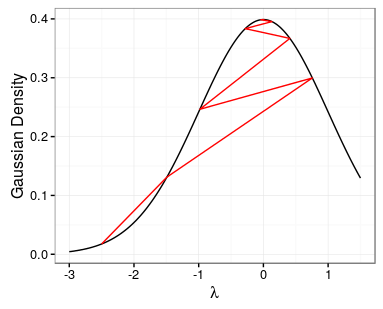
\includegraphics[width = 0.4\textwidth]{gradientascent}
\end{figure}
\item \hyperlink{VB}{Return}
\end{itemize}
\end{frame}

\end{document}